\documentclass[a4j,12pt]{jreport}

\usepackage{tex/mthesis}
\usepackage{amsmath,amssymb,ascmac}
\usepackage[cmbtt]{bold-extra}
\usepackage[dvipdfmx]{graphicx}
\usepackage{stmaryrd} % for llbracket and rrbracket

% for source code in the document
\usepackage{listings}
\usepackage{color}
\usepackage[scaled=0.95]{inconsolata}
\usepackage{framed}


% SFRP syntax
\lstdefinelanguage{SFRP}{
  morekeywords={in,from,out,init,import,as,op,type,let,where,case,of,if,then,else,foreign,ptype,infix,infixl,infixr},
  morecomment=[l]{--}
}
\renewcommand{\lstlistingname}{Code}

% source code coloring
% cf. https://www.sharelatex.com/learn/Code_listing
\definecolor{codegreen}{rgb}{0.1,0.6,0.3}
\definecolor{codegray}{rgb}{0.5,0.5,0.5}
\definecolor{codepurple}{rgb}{0.58,0,0.82}
\definecolor{codered}{rgb}{0.6,0.1,0.2}
\definecolor{backcolour}{rgb}{0.95,0.95,0.92}
\lstdefinestyle{mystyle}{
%    backgroundcolor=\color{backcolour},
    commentstyle={\color{codegreen}},
    keywordstyle={\bfseries\color{codered}},
    numberstyle={\tiny\color{codegray}},
    stringstyle={\color{codepurple}},
    basicstyle={\ttfamily},
    breakatwhitespace=false,
    breaklines=true,
    captionpos=b,
    keepspaces=true,
    numbers=left,
    numbersep=5pt,
    showspaces=false,
    showstringspaces=false,
    showtabs=false,
    tabsize=2,
    frame=single,
    xleftmargin=1.2em
}
\lstset{style=mystyle}


\年度{平成28年度}
\提出年月{平成29年1月}
\題名{マイクロコントローラための実用的な \\ 関数リアクティブプログラミング言語}
\指導教員名{渡部卓雄}
\職名{教授}
\研究科{情報理工学}
\専攻{計算工学}
\学籍番号{15M38224}
\氏名{澤田賢祐}
\内容梗概{本研究の目的は、豊富なメモリ資源を持たないマイクロコントローラ上で動作させることが可能な、
記述性に優れた独自の関数リアクティブプログラミング(FRP)言語の設計手法を提案することである。
FRPは入出力の相互作用を宣言的に記述することによってソフトウェアの動作を表現するプログラミング手法であり、
非同期的に発生するイベントに反応し何らかの処理を行うプログラムを簡潔に記述することができる。
GUIアプリケーションのフロントエンド開発等の領域では既に広く実用化されている一方で、
小規模組込みシステム開発等の計算資源に制約を抱える領域においては、現在までにあまり実用化されて来なかった。
これは、従来のFRP言語やFRPフレームワークは豊富なメモリ資源を活用する形で実現されており、
マイクロコントローラ等の豊富なメモリ資源を持たない環境において適用することが難しいためである。

本研究では、FRPの優れた表現性能は必ずしも豊富なメモリ資源の活用を前提として成り立っているわけでは無いことを明らかにする
ために、僅かなメモリ使用量で動作する独自のFRP言語{\it SFRP}を設計及び実装した。
SFRPはメモリ制約環境下において避けるべき動的メモリ確保を完全に排したプログラミング言語でもあり、
C言語コンパイラがサポートされるマイクロコントローラ上で動作させることができる。

本論文では、SFRPが採用するFRPの計算モデルを示し、如何にして省メモリ性を実現しているのかを述べると共に、
SFRPとマイクロコントローラを用いた実用的な小規模組込みシステムの開発手順についても例示する。
同時にSFRPの空間的・計算量的な性能評価についても行い、記述性と実用性についても議論する。
}

\begin{document}
\maketitle
\setcounter{page}{1}
\renewcommand{\thepage}{\roman{page}}
\setcounter{tocdepth}{1}
\tableofcontents
\clearpage
\setcounter{page}{1}
\renewcommand{\thepage}{\arabic{page}}
\renewcommand\thefootnote{*\arabic{footnote}}
\chapter{序論}
\section{研究の目的と背景}
\section{本論文の構成}
\cite{suzuki2016cfrp}

\chapter{背景知識}
\section{関数リアクティブプログラミング}
\section{マイクロコントローラと小規模組込みシステム}

\chapter{言語デザイン}\label{sec:language}
本研究では、記述性と省メモリ実行性を重視した組込みシステム向けFRP言語{\it SFRP}を設計した。
本章では、まず\ref{sec:language:model}節において、SFRPがどのような計算モデルに従うプログラミング言語であるのかを説明する。
続く\ref{sec:language:syntax}節では、SFRPの構文と言語仕様について示す。
最後に\ref{sec:language:memory}節において、SFRPの実行時に必要とされるメモリ使用量を評価する手法を提示する。

\section{SFRPの計算モデル}\label{sec:language:model}
本節では、具体的な構文には触れることなく、SFRPがどのようなプログラミング言語であるかについての解説を行う。
まず\ref{sec:language:model:program}項において、SFRPがどのようにシステムを表現するプログラミング言語であるのかを説明する。
続く\ref{sec:language:model:execution}項では、SFRPプログラムがどのように実行されるのかを示す。
さらに\ref{sec:language:model:validation}項において、プログラムの実行可能性について述べる。

\subsection{プログラムの表現}\label{sec:language:model:program}
SFRPプログラムは、時刻によって変動する値(時変値、time-varying value)によって構成される。
一つのSFRPプログラムは、入力時変値を前提とした出力時変値の定義であると言える。

以下に、SFRPにおいて時変値がどのように表現され、ユーザはどのような形で時変値を定義することができるのかを述べていく。

\begin{itemize}
  \item
  時変値は時刻$t$をパラメータに取る関数とみなされる。
  \begin{equation*}
    Time \rightarrow Value
  \end{equation*}

  \item
  時刻$t$におけるプログラムへの入力は、プリミティブな時変値
  \footnote{他の時変値を用いて定義されるのではなく、前提として与えられる時変値をプリミティブな時変値と呼ぶ。}
  として表現される。
  \begin{equation*}
    {\it input} \, :: \, Time \rightarrow Value
  \end{equation*}

  \item
  他の時変値を参照して演算を加えることにより、新たな時変値を定義することができる。
  たとえば、時変値Aの値と時変値Bの値の和を取る時変値Cを定義することができる。
  \begin{equation*}
    C(t) := A(t) + B(t)
  \end{equation*}

  \item
  各時変値は、時刻$t$における値(現在値)の参照と、微小時間$ \Delta t(t) $前の値(直前値)の参照が許されている。
  たとえば、時変値Aの現在値と時変値Bの直前値の和を取る時変値Dを定義することができる。
  \begin{equation*}
    D(t) := A(t) + B(t - \Delta t(t))
  \end{equation*}

  \item
  $ \Delta t $は微小時間を表すプリミティブな時変値である。
  \begin{equation*}
    \Delta t(t) > 0
  \end{equation*}

  \item
  初期値($ t < 0 $における値)を特別に指定した時変値を定義することができる。
  たとえば、$t \geq 0$においては時変値Aの値を取り、$t < 0$においては0を取る時変値Bを定義することができる。
  \begin{equation*}
    B(t) := \begin{cases}
      A(t) & (t \geq 0) \\
      0 & (t < 0)
    \end{cases}
  \end{equation*}

  \item
  時刻$t$におけるプログラムの出力は、任意の時変値によって定義される。
  以下は、時変値Dの現在値に1を加えた時変値を出力とする例である。
  \begin{equation*}
    output(t) := D(t) + 1
  \end{equation*}
\end{itemize}

\subsection{プログラムの実行}\label{sec:language:model:execution}
\ref{sec:language:model:program}項にて示したプログラム表現は、 以下に示す逐次的操作によって実行される。
\begin{screen}
\begin{enumerate}
  \item $ {\it timestamp}^{\prime} := 現在時刻$
  \item $ {\it timestamp} := 現在時刻 (> timestamp^{\prime})$
  \item $ {\it elapsed} := {\it timestamp} - {\it timestamp}^{\prime} $
  \item $\tau$が未定義であるなら$ \tau := 0 $として、そうでないなら$ \tau := \tau + {\it elapsed} $とする。
  \item $ \Delta t(\tau) := {\it elapsed} $
  \item 入力を受け取り、$ {\it input}(\tau) $の値とする。
  \item プログラム中の全ての時変値の、$t=\tau$における値を求める。
  \item $ {\it output}(\tau) $の値を出力する。
  \item $ {\it timestamp}^{\prime} := {\it timestamp} $
  \item 2に戻る。
\end{enumerate}
\end{screen}

\subsection{プログラムの実行可能性}\label{sec:language:model:validation}
あるプログラムに対し、\ref{sec:language:model:execution}項の操作が途中で失敗すること無く適用可能であるとき、
そのプログラムは実行可能であるとここでは言う。
\ref{sec:language:model:execution}項の操作において失敗する可能性が考えられるのは、7番目の処理(処理7)である。
ただし入出力の処理と、数値に対する演算処理は必ず成功すると仮定する。
本項では、処理7が成功するための条件について議論を行う。

${\it output}(\tau)$の値の計算過程において、存在しない時変値が参照される場合は当然の事ながら処理7は実行不可能である。
以下では、存在しない時変値への参照はプログラム中に含まれないと仮定する。
また、時変値の参照による依存関係に循環は無いと仮定する。
ただし時変値Aが時変値Bの現在値を参照して定義されているときに限り、AはBに依存すると見なす。

$\tau = a(\neq 0)$において処理7が実行される場合、
過去の$\tau = a - \Delta t(a)$である場合において処理7の実行に成功しているはずである。
したがって、プログラム中の任意の時変値$v$について、直前値である$v(\tau - \Delta t(\tau))$は計算可能である。
このことから補題1が成り立つ。
\begin{itembox}[l]{補題1}
  $\tau = 0$のとき処理7の実行に成功する $\Longleftrightarrow$ 常に処理7の実行に成功する
\end{itembox}

$\tau < 0$において処理5および処理6が行われることはないため、
任意の$a < 0$について、input(a)および$\Delta t(a)$は未定義となる。
また、$\tau = 0$のとき
\begin{center}
  $\tau - \Delta t(\tau) = -\Delta t(0) < 0$
\end{center}
である。
この2点から、$\tau = 0$のとき時変値inputの直前値である$input(\tau - \Delta t(\tau))$
および時変値$\Delta t$の直前値である$\Delta t(\tau - \Delta t(\tau))$は未定義となると分かる。
また、現在値あるいは直前値が未定義となる場合が存在する時変値は、inputと$\Delta t$の他に存在しない。
このことから補題2が成り立つ。
\begin{itembox}[l]{補題2}
  $\tau = 0$のとき処理7の実行に成功する $\Longleftrightarrow$ \\
  プログラム中に、時変値${\it input}$あるいは$\Delta t$に対する直前値参照が存在しない。
\end{itembox}

補題1および補題2から、プログラムの実行可能性について以下が成り立つ。
\begin{screen}
  プログラムが実行可能である $\Longleftrightarrow$ \\
  プログラム中に、時変値${\it input}$あるいは$\Delta t$に対する直前値参照が存在しない。
\end{screen}

このことから、時変値$input$および$\Delta t$の初期値($t < 0$における値)が特別に定義されていれば、
プログラムは必ず実行可能であるということも分かる。


\section{SFRPの構文と言語仕様}\label{sec:language:syntax}
\subsection{外部ノードの定義}
トップレベルに名前付きで定義されるプリミティブな時変値を外部ノード(入力ノード)と呼ぶ。
これは、\ref{sec:language:model}節で述べた${\it input}$に相当する。
外部ノードを定義するために用いるのが、外部ノード定義構文である。
外部ノード定義構文では、入力値を取得する関数の名前(および引数の式)と共に外部ノードが定義される。
以下は入力関数\texttt{\$getInput()}によって値が供給される外部ノード\texttt{@input}を定義する例である。
\begin{lstlisting}[basicstyle=\ttfamily\small,language=SFRP]
in @input from $getInput()
\end{lstlisting}
ノードの名前は\texttt{@}から開始されなければならないことに注意されたい。
以下のように初期値を設定することもできる。
ただし、初期値の定義式において他の時変値を参照することはできない
\footnote[1]{
\ref{sec:language:model}節で示した計算モデルにはない非本質的な制約であり、
将来的にはこの制約が必要ない形に言語仕様が変更される可能性がある。
}。
\begin{lstlisting}[basicstyle=\ttfamily\small,language=SFRP]
in @input init 0 from $getInput()
\end{lstlisting}
\ref{sec:language:model}節では入力時変値が一つであるとして述べたが、
プログラム中に複数の外部ノードを定義することも可能である。
\begin{lstlisting}[basicstyle=\ttfamily\small,language=SFRP]
in @input1 from $getInput1()
in @input2 from $getInput2(@input1)
\end{lstlisting}

\subsection{内部ノードの定義}
トップレベルに名前付きで定義されたプリミティブでない時変値を内部ノードと呼ぶ。
この内部ノードを定義するために用いるのが、内部ノード定義構文である。
以下は内部ノード定義構文の使用例である。
外部ノードの場合と同様に、初期値の定義式において他の時変値を参照することはできない。
\begin{lstlisting}[basicstyle=\ttfamily\small,language=SFRP]
@a = 0
@b = @a + 1
@c init 0 = @b + @@c
\end{lstlisting}
これら3つの内部ノード定義は、それぞれ以下の時変値定義に相当する。
\begin{equation*}
  a(t) := 0
\end{equation*}

\begin{equation*}
  b(t) := a(t) + 1
\end{equation*}

\begin{equation*}
  c(t) := \begin{cases}
    b(t) + c(t-\Delta(t)) & (t \geq 0) \\
    0 & (t < 0)
  \end{cases}
\end{equation*}
直前値の参照が許されているのは、初期値が定義されたノードのみであることに注意されたい \footnotemark[1]。

\subsection{ノード出力の定義}
ノードを用いて出力を定義するために用いるのが、ノード出力定義構文である。
ノード出力定義構文では、値を出力する関数の名前(および引数の式)が定義される。
以下は出力定義構文の使用例である。
\begin{lstlisting}[basicstyle=\ttfamily\small,language=SFRP]
out $setOutput(@foo, @bar + 1)
\end{lstlisting}
\ref{sec:language:model}節においては出力値は${\it output}(t)$なる時変値として表現されると述べた。
ノード出力定義構文においては、そのように出力時変値を単一の値としてまとめる必要はなく、複数の時変値を出力関数に与える形で出力を定義することができる。
また、ノード出力は複数定義することができる。
\begin{lstlisting}[basicstyle=\ttfamily\small,language=SFRP]
out $setOutput1(@foo)
out $setOutput2(@bar)
\end{lstlisting}

\subsection{関数の定義}
トップレベルに名前付きの関数を定義するために用いるのが、関数定義構文である。
定義式内においてノードを参照することはできない \footnotemark[1]。
以下は関数定義構文の使用例である。
\begin{lstlisting}[basicstyle=\ttfamily\small,language=SFRP]
sum(a, b) = a + b
\end{lstlisting}
副作用を含む関数(I/O関数)を定義する場合、その関数の名前は\texttt{\$}から開始されなければならない。
\begin{lstlisting}[basicstyle=\ttfamily\small,language=SFRP]
$setOutputDouble(x) = $setOutput(x * 2)
\end{lstlisting}
また、I/O関数を使用することができるのは、以下の3つの場合のみである。
\begin{itemize}
  \item 他のI/O関数の定義式内において関数呼び出しを行う場合
  \item 外部ノード定義構文において指定する場合
  \item ノード出力定義構文において指定する場合
\end{itemize}
通常関数・I/O関数共に、再帰的な関数を定義することは認められていない。
これは、省メモリ実行性およびリアルタイム性の達成の観点から課される制約である。

\subsection{演算子の定義}
演算子を定義するために用いるのが、演算子定義構文である。
以下は、左辺の値を無視して右辺の値を取る演算子\texttt{>->}を定義する例である。
\begin{lstlisting}[basicstyle=\ttfamily\small,language=SFRP]
op >->(a, b) = b
\end{lstlisting}
\texttt{infix}構文を用いて演算子の結合性および優先順位を定義することができる。
\begin{lstlisting}[basicstyle=\ttfamily\small,language=SFRP]
infixl >-> 0
infixr >-> 0
infix >-> 0
\end{lstlisting}
それぞれ左結合、右結合、非結合を指定する文である。当然ならが一つの演算子に対して一つの指定のみが認められる。

\subsection{外部関数の定義}
C言語によって定義された外部関数をSFRPプログラム内で使用するために用いるのが、外部関数定義構文である。
以下は、c言語で定義された関数\texttt{func\_in\_c}を、SFRPにおいて関数\texttt{funcInSFRP}として定義する例である。
\begin{lstlisting}[basicstyle=\ttfamily\small,language=SFRP]
foreign func_in_c as funcInSFRP(Int, Int) : Int
\end{lstlisting}
ここでは、関数\texttt{funcInSFRP}は\texttt{Int}型の引数を2つ取って\texttt{Int}型の値を返す関数として定義されている。
また、C言語で定義された関数が副作用を含む場合、SFRPにおける関数名は\texttt{\$}から開始されなければならない。
C言語のオペレータを外部関数(演算子)として定義することも可能である。
\begin{lstlisting}[basicstyle=\ttfamily\small,language=SFRP]
foreign + as +(Int, Int) : Int
\end{lstlisting}

\subsection{外部ファイルのimport}
外部ファイルをインポートするために用いるのが、import構文である。
以下はSFRPの標準ライブラリをインポートする例である。
\begin{lstlisting}[basicstyle=\ttfamily\small,language=SFRP]
import Base
\end{lstlisting}
この例では、標準ライブラリにて定義された関数等の名前がそのまま現在のファイルにおいて使用可能となる。
以下のように修飾名を指定して外部ファイルをインポートすることもできる。
\begin{lstlisting}[basicstyle=\ttfamily\small,language=SFRP]
import Base.STDIO as IO
\end{lstlisting}
この場合、\texttt{Base.STDIO}にて定義された名前は、\texttt{IO.}をプレフィックスに付けて参照することができる。

\subsection{代数的データ構造の定義}
多相的な代数的データ構造を定義するために用いるのが、type構文である。
以下は典型的な3種類の代数的データ構造を定義する例である。
\begin{lstlisting}[basicstyle=\ttfamily\small,language=SFRP]
type Bool = False | True
type Tuple2[a, b] = Tuple2(a, b)
type Maybe[a] = Nothing | Just(a)
\end{lstlisting}
再帰的なデータ構造の定義は認められていない。
すなわち、以下のようなデータ構造を定義することはできない。
\begin{lstlisting}[basicstyle=\ttfamily\small,language=SFRP]
type List(a) = Empty | Cons(a, List(a))
\end{lstlisting}
これは省メモリ実行性を実現するための制約であり、\ref{sec:language:model}節における計算モデルと直接関係はない。

\subsection{型システムと型アノテーション}
SFRPはMLに近い形式の多相的な型システムを採用する。
多相性が認められるのは代数的データ構造定義および関数定義のレベルにおいてのみであり、局所変数およびノードの多相性は認められていない。
すなわち、以下のような記述は型エラーとなる。
\begin{lstlisting}[basicstyle=\ttfamily\small,language=SFRP]
@x : (Maybe[Int], Maybe[Bool]) = (x, x) where x = Nothing
\end{lstlisting}
関数定義、演算子定義、ノード定義には型アノテーションを付記することができる。
以下はそれぞれの記述例である。
\begin{lstlisting}[basicstyle=\ttfamily\small,language=SFRP]
fromMaybe(x : a, m : Maybe[a]) : a =
  case m of
    Nothing -> x
    Just(x) -> x

op >->(x : a, y : b) : b = y

@a : Int = 0
@b init 0 : Int = @@b + 1
\end{lstlisting}
ただし型アノテーションに型変数を用いる場合、全称束縛ではなく存在束縛となる。
すなわち、以下のような記述は型エラーとはならない。
\begin{lstlisting}[basicstyle=\ttfamily\small,language=SFRP]
@x : a = 0
\end{lstlisting}


\subsection{式}
SFRPにおいて利用可能な式の種類を示す。
\begin{itemize}
\item let式\\局所変数を導入することができる。代入群はオフサイドルールによってブロック化される。
左辺にはパターンを置くことができる。
\begin{lstlisting}[basicstyle=\ttfamily\small,language=SFRP]
let x = 0
    (y,z) = (1, 2) in
  x + y + z
\end{lstlisting}
where節を用いて他の代入節(\texttt{=<exp>}の形をとる節)に付加する形でも局所変数を導入することができる。
代入群はオフサイドルールによってブロック化される。
\begin{lstlisting}[basicstyle=\ttfamily\small,language=SFRP]
@a = x + y where
  x = 1
  y = 2
\end{lstlisting}

\item case式\\パターンマッチを行うことができる。パターン群はオフサイドルールによってブロック化される。
パターン群の網羅性がチェックされ、非網羅的である場合は不正な式とみなされる。
必ずマッチするパターンとして変数あるいはアンダースコア\texttt{\_}を用いることができる。
\begin{lstlisting}[basicstyle=\ttfamily\small,language=SFRP]
case x of
  Nothing -> (0, Nothing)
  Just(a) as b -> (a, b)
\end{lstlisting}

\item if式
\begin{lstlisting}[basicstyle=\ttfamily\small,language=SFRP]
if x == 1 then x else y
\end{lstlisting}

\item 関数・演算子の適用式
\begin{lstlisting}[basicstyle=\ttfamily\small,language=SFRP]
f(1 + 1)
\end{lstlisting}

\item 代数的データ構造のコンストラクタの呼び出し式\\
タプルの糖衣構文がサポートされる。
たとえば、\texttt{(1,2)}は\texttt{Tuple2(1,2)}の別表記である。
\begin{lstlisting}[basicstyle=\ttfamily\small,language=SFRP]
Just(1)
(1, 2)
\end{lstlisting}

\item 局所変数、ノードの現在値・直前値の参照式
\begin{lstlisting}[basicstyle=\ttfamily\small,language=SFRP]
foo
@bar
@@bar
\end{lstlisting}
\end{itemize}


\section{メモリ使用量の評価}\label{sec:language:memory}
組込みシステム開発では多くの場合、プログラムが消費するメモリ使用量を何らかの形で見積もる必要がある。
メモリ不足によってプログラムが異常終了する可能性は極力排除しなければならないためである。

SFRPではこの見積もりを容易にするため、全てのデータ構造の実体を静的領域に確保できるように設計されている。
すなわち、データ構造をコールスタックに積んだり、ヒープ上に動的確保したりせずとも実行できるように設計されている。

データ構造の実体を静的領域に確保するためには、同時に使用されるデータ構造の最大量が静的に特定可能でなければならない。
SFRPは再帰的なデータ構造と関数を排除することによって、この最大量を静的に計算可能としている。

図\ref{fig:memory-eval}に示すのは、SFRPプログラムによって同時に使用されるデータ構造の最大量を評価する式である。
図における値$memory$がこの最大量を表す。

ただしこの評価はデータ構造の確保に必要なメモリ量についてのみを対象としており、
プログラムの実行に必要な全体のメモリ量についての評価ではないことに注意されたい。
すなわち、局所変数の使用や(非再帰的な)関数呼び出しに必要なメモリ量はまた別に存在する。
ただしこちらのメモリ使用量についても、SFRPにおいては関数呼び出しが非再帰的であるため、理論上はその最大量を求めることができる
\footnote{
現状のSFRP実装ではバイナリを直接生成しないため、こちらの上限値の評価を具体的に行うことは難しい。
}。


\begin{figure}[p]
\begin{framed}
  プログラムにおけるデータ構造のメモリ使用量 \vspace{10pt}

  \begin{math}
    memory \ := \
    \sum_{T \ \in \ EmergedTypes} memorysize(T) * whole_T
  \end{math}
  \vspace{25pt}

  プログラムにおけるデータ構造Tの使用量 \vspace{10pt}

  \begin{math}
    whole_T \ := \
    \max \{init_T, cycle_T\}
  \end{math}
  \vspace{10pt}

  \begin{math}
    init_T \ := \
    \sum_{n \ \in \ InitializedNodes} \llbracket initexp(n) \rrbracket _T
  \end{math}
  \vspace{10pt}

  \begin{math}
    cycle_T \ := \
    \sum_{n \ \in \ InitializedNodes} \llbracket type(n) \rrbracket _T
    \ + \
    \sum_{n \ \in \ InnerNodes} \llbracket exp(n) \rrbracket _T
  \end{math}
  \vspace{25pt}

  式におけるデータ構造Tの使用量 \vspace{10pt}

  \begin{math}
    \llbracket \texttt{let} \ p_1 = e_1 \ ; \ \cdots \ ; \ p_n = e_n \ \texttt{in} \ e\rrbracket _T
    \ \rightarrow \
    \llbracket e \rrbracket _T + \sum^n_{i=1} \llbracket e_i \rrbracket _T
  \end{math}
  \vspace{10pt}

  \begin{math}
    \llbracket \texttt{case} \ e \ \texttt{of} \ p_1 \rightarrow e_1 \
    ; \ \cdots \ ; \ p_n \rightarrow e_n \rrbracket _T
    \ \rightarrow \
    \llbracket e \rrbracket _T + \max \{ \llbracket e_i \rrbracket _T, i = 1, \cdots, n \}
  \end{math}
  \vspace{10pt}

  \begin{math}
    \llbracket \texttt{if} \ e_1 \ \texttt{then} \ e_2 \ \texttt{else} \ e_3 \rrbracket _T
    \ \rightarrow \
    \llbracket e_1 \rrbracket _T + \max \{ \llbracket e_2 \rrbracket _T, \llbracket e_3 \rrbracket _T \}
  \end{math}
  \vspace{10pt}

  \begin{math}
    \llbracket function(e_1, \cdots, e_n) \rrbracket _T
    \ \rightarrow \
    \llbracket body(function) \rrbracket _T + \sum^n_{i=1} \llbracket e_i \rrbracket _T
  \end{math}
  \vspace{10pt}

  \begin{math}
    \llbracket constructor(e_1, \cdots, e_n) \rrbracket _T
    \ \rightarrow \
    \sum^n_{i=1} \llbracket e_i \rrbracket _T +
    \begin{cases}
      1 & (type(constructor) \ = \ T) \\
      0 & (type(constructor) \ \neq \ T)
    \end{cases}
  \end{math}
  \vspace{10pt}

  \begin{math}
    \llbracket \texttt{foo} \rrbracket _T \ \rightarrow \ 0
  \end{math}
  \vspace{10pt}

  \begin{math}
    \llbracket \texttt{@bar} \rrbracket _T \ \rightarrow \ 0
  \end{math}
  \vspace{10pt}

  \begin{math}
    \llbracket \texttt{@@bar} \rrbracket _T \ \rightarrow \ 0
  \end{math}
  \vspace{25pt}

  型におけるデータ構造Tの使用量 \vspace{10pt}

  \begin{math}
    \llbracket
      type
    \rrbracket _T
    \ \rightarrow \
    \begin{cases}
      1 & (type \ = \ T) \\
      \max \{ \llbracket c \rrbracket, \ c \ \in \ constructors(type) \} & (type \ \neq \ T)
    \end{cases}
  \end{math}
  \vspace{10pt}

  \begin{math}
    \llbracket
      constructor(type_1, \ \cdots, type_n)
    \rrbracket _T
    \ \rightarrow \
    \sum^n_{i=1} \llbracket type_i \rrbracket _T
  \end{math}
  \vspace{10pt}
\end{framed}
\caption{プログラムがデータ構造を確保するために必要なメモリ量の評価}
\label{fig:memory-eval}
\end{figure}


\chapter{実装}
本研究ではリファレンス実装として、C言語を中間表現とするSFRPのコンパイラ
\footnote{https://github.com/sfrp/sfrp}を作成した。
以降ではこの実装をSFRPコンパイラと呼称する。
本章では、SFRPコンパイラによってプログラムがどのように実行されるのかを説明する。

\section{SFRPプログラム例}
以降の節では、Code \ref{code:sample}に示す簡単なSFRPのプログラムBLINKLEDを例にとって解説および評価を行う。
このプログラムは、接続されたLEDの明滅を一定周期で切り替えるシステムを記述したものである。

マイクロコントローラには8KBのFlashと1KBのRAM、16MHzの内部クロックを持つAtmel AVR 8ビットマイクロコントローラ ATmega8
\footnote{http://www.atmel.com/ja/jp/devices/ATMEGA8.aspx}
を使用し、汎用入出力ポートPD7とGNDの間にLEDを接続する。
本来、I/O処理のインターフェースはアーキテクチャ毎に個別にユーザが定義する必要があるが、
本マイクロコントローラATmega8についてはリファレンス実装としてI/O処理がSFRPの標準ライブラリに組み込まれている。

\newpage
\lstinputlisting[language=SFRP,tabsize=2,caption={SFRPの例題プログラム(BLINKLED)},label={code:sample}]{./code/simple-example/BlinkLED.sfrp}


\section{実行過程}
SFRPコンパイラによって、BLINKLEDは以下の繰り返し処理として実行される。
これは、\ref{sec:language:model:execution}項における実行モデルに基づいている。
\begin{figure}[h]
\begin{screen}
\begin{enumerate}
  \item 全ての初期値付きノードの初期値が計算され、初回の直前値として保持される。
    BLINKLEDの場合、初期値付きノードは\texttt{@led}のみである。
  \item 依存関係の順に従い、全てのノードの現在値が導出される。
    BLINKLEDの場合、入力ノードは存在せず、内部ノードも\texttt{@led}のみであるため、
    \texttt{@led}の現在値が計算されるのみである。
  \item ノード出力定義に従い、出力を行う。
    BLINKLEDの場合、13行目のノード出力定義に従い、
    \texttt{@led}の現在値がOnであるなら出力ポートPD7にTrue(High)が出力され、OffであるならFalse(Low)が出力される。
  \item 初期値付きノードの現在値は次回の計算フェーズまで保持され、次回の直前値として参照される。
    BLINKLEDの場合、\texttt{@led}の現在値が次回まで保持される。
  \item 2に戻る。
\end{enumerate}
\end{screen}
\caption{BLINKLEDの実行処理}
\label{fig:imp:exec}
\end{figure}

\section{式や関数の表現}
SFRPの式や関数とC言語の式や関数の間にギャップはあまりないため、特に複雑な変換処理などは介さずにC言語へとコンパイルされる。
let式で導入される局所変数はその式が所属する関数の局所変数として巻き上げられ、パターンマッチ式やif式は3項演算子へと変換される。
関数呼び出しおよびコンストラクタ呼び出しはそのまま対応する関数の呼び出し式として表現される。
内部ノードは関数として表現され、依存する他のノードの参照は関数のパラメータを介して行われる。

\section{データ構造の確保と取り扱い}
SFRPコンパイラはデータ構造の実体を静的領域に確保し、実行時にはポインタを介してデータ構造を参照する。
ノードの現在値演算が一巡する毎(図\ref{fig:imp:exec}の第5項目を実行する毎)に全データ構造の参照到達性が調べられ、使用されていないデータ構造は再利用される。
このとき、初期値付きノードの現在値がルートとなって参照到達性の判定が行われる。

静的表域に確保するされるデータ構造の実体の必要数は図\ref{fig:memory-eval}の評価によって求めることができる。
BLINKLEDの場合、\texttt{Blink}型のデータ構造に対して必要な実体は2つである。


\section{実行時性能}
本研究ではBLINKLEDの実行時性能を調査し、SFRP言語およびSFRPコンパイラの簡易的な実行性能評価とする。

\subsection{メモリ性能}
avr-gcc(v4.9.2)を用いてバイナリ(実行形式)を生成し、この実行形式を分析することによってメモリ使用量の算出を行う。
ただしコードサイズを小さくするため、以下のコンパイルオプションを指定した。
\begin{lstlisting}[basicstyle=\ttfamily\small,numbers=none,frame=none]
-Os -fdata-sections -ffunction-sections -Wl,--gc-sections
\end{lstlisting}
2つ目以降のオプションは不要な関数定義をバイナリに含めないようにするための指定である。

SFRPコンパイラが出力したC言語コードを元に関数コールグラフを作成すると図\ref{fig:imp:call_graph}に示す通りとなる。
ただし関数名の右横の数字はその関数で導入される局所変数のバイトサイズである。
このサイズはgccにオプション\texttt{-fstack-usage}を指定することで求めることができる。
1回の関数呼び出しで消費するスタック領域を
\begin{center}
$スタックポインタを格納する2バイト領域 + 局所変数を格納する領域$
\end{center}
であると仮定すると、図\ref{fig:imp:call_graph}より最大スタックサイズは
\begin{center}
$ (2 + 6) + (2 + 0) + (2 + 2) + (2 + 0) = 16 byte$\\
\end{center}
であると算出される。

プログラムサイズおよび静的領域の使用量についてはavr-sizeコマンドによってそのまま求めることができる。
以上を纏めると表\ref{fig:imp:size}に示す通りとなり、
BLINKLEDのFlushの使用量は$486byte$、RAMの最大使用量は$24byte$であると算出される。

\begin{figure}[h]
 \begin{center}
  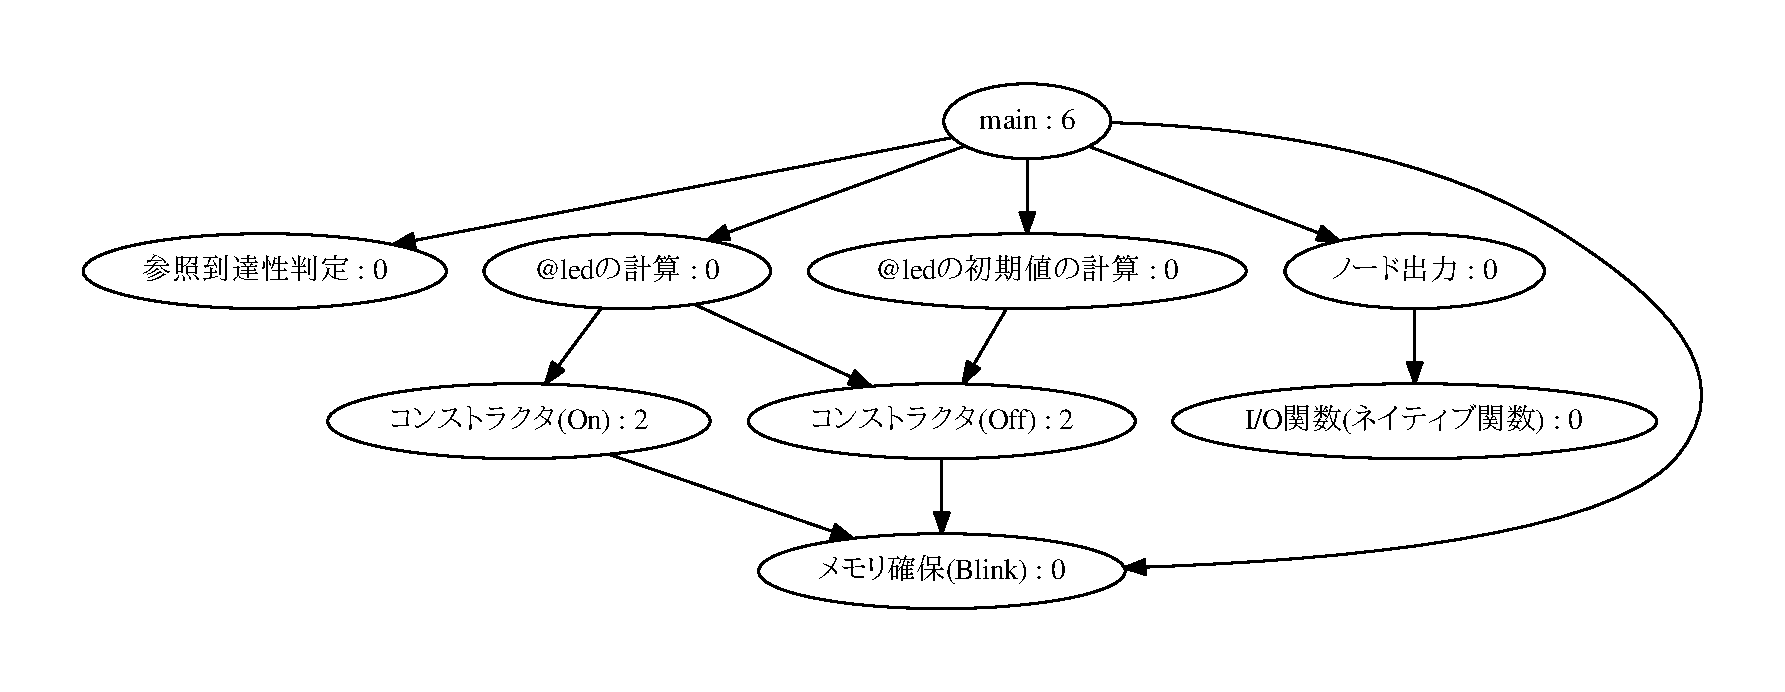
\includegraphics[width=160mm]{figure/call_graph.pdf}
 \end{center}
 \caption{BLINKLEDをコンパイルした結果の関数コールグラフ}
 \label{fig:imp:call_graph}
\end{figure}

\begin{table}[h]
  \centering
  \begin{tabular}{l|r}
    textサイズ(avr-sizeコマンドより) & 486 byte \\ \hline
    dataサイズ(avr-sizeコマンドより) & 0 byte \\ \hline
    bssサイズ(avr-sizeコマンドより)  & 8 byte \\ \hline
    最大スタックサイズ(-fstack-usageオプションおよび手計算により算出)  & 16 byte \\ \hline
  \end{tabular}
\caption{BLINKLEDのメモリ使用量}
\label{fig:imp:size}
\end{table}


\subsection{速度性能}
メモリ性能の評価と同じ条件で実行形式を生成し、ATmega8実機上で実際にプログラムを動かして実行速度を計測する。
実行速度はLEDの明滅切り替え(すなわち、出力のHigh/Lowの切り替え)の間隔を測定することによって求める。
この測定を、実時間計測が可能なもう1つのマイクロコントローラを接続することによって行ったところ、結果は表\ref{fig:imp:time1}の通りとなった。

\begin{table}[h]
  \centering
  \begin{tabular}{c}
    $ \input{code/simple-example/evaluator/result1.txt}ms$ \\ \hline
  \end{tabular}
\caption{BLINKLEDのLED明滅が切り替わる時間の間隔(20回平均)}
\label{fig:imp:time1}
\end{table}

プログラムBLINKLEDにおいて10000回のイテレーションを経てLEDの明滅が切り替わることから、
イテレーション1回(図\ref{fig:imp:exec}の一巡)に対して平均
$ \input{code/simple-example/evaluator/result2.txt} \mu s$
の計算時間を要していることがわかる。

イテレーション1回の計算に要する時間は当然プログラムに依存する。
しかしSFRP言語が再帰的関数の定義を認めていないことを考慮すれば、計算時間は概ねコードの分量に比例するであろうと予測できる。
従ってBLINKLEDよりも複雑でより実用的なプログラムを記述したとしても、イテレーション1回に要する時間はせいぜいこれの数倍から十数倍程度
(すなわち$1ms$から$10ms$程度)に収まるものと思われる。
この程度の所要時間であれば、多くの小規模組込みシステムにとっては十分な反応速度を得られるであろう。

\chapter{実例研究}
本章では実例研究として、オーソドックスかつ単純な機能を持つキッチンタイマー(カウントダウンタイマー)の開発を行う。
これはソフトウェア的な複雑さを持つ小規模組込みシステムの典型的な例であり、SFRPが第一にターゲットとする類のシステムである。

\section{アプリケーションの仕様}
開発対象となるキッチンタイマー(KTIMER)の機能仕様を図\ref{fig:ktimer:spec}に簡単に示す。
この仕様に基づいて包括的な状態遷移図を作成すると図\ref{fig:ktimer:state}の様になる。

図\ref{fig:ktimer:state}において、四角形のテーブル3つがそれぞれアプリケーションの状態を表す。
各テーブルの1段目は状態名、2段目は状態変数の一覧、3段目はその状態におけるアプリケーションの動作を示している。
テーブル同士を繋ぐ矢印は状態遷移を表し、これに付属する文字列は遷移条件(角括弧の中)と遷移後の状態変数の値を示している。
また、左上に存在する中空からの矢印はアプリケーションの開始(停止状態からの遷移)を表している。


\begin{figure}[h]
\begin{screen}
\begin{itemize}
  \item 分と秒を2桁ずつ表示する表示器、ボタンA、ボタンB、ボタンC、ブザーを備える。
  \item 電源を投入すると、分数と秒数が共に0で一時停止した状態となる。
  \item 一時停止中にボタンCを押すとカウントダウンを開始する。ただし分数と秒数が共に0の場合は何もしない。
  \item 一時停止中にボタンAを押すと分数がカウントアップされる。ただし分数が99の場合は0に戻る。
  \item 一時停止中にボタンBを押すと秒数がカウントアップされる。ただし秒数が59の場合は0に戻る。
  \item 一時停止中にボタンAとBを同時に押すと分数と秒数が共に0にリセットされる。
  \item カウントダウン中にボタンCを押すと一時停止する。
  \item カウントダウンが0に達するとブザーが鳴る。
  \item ブザーが鳴っている時にボタンCを押すとブザーは停止し、分数と秒数が共に0で一時停止した状態になる。
\end{itemize}
\end{screen}
\caption{KTIMERの機能仕様}
\label{fig:ktimer:spec}
\end{figure}

\begin{figure}[h]
 \begin{center}
  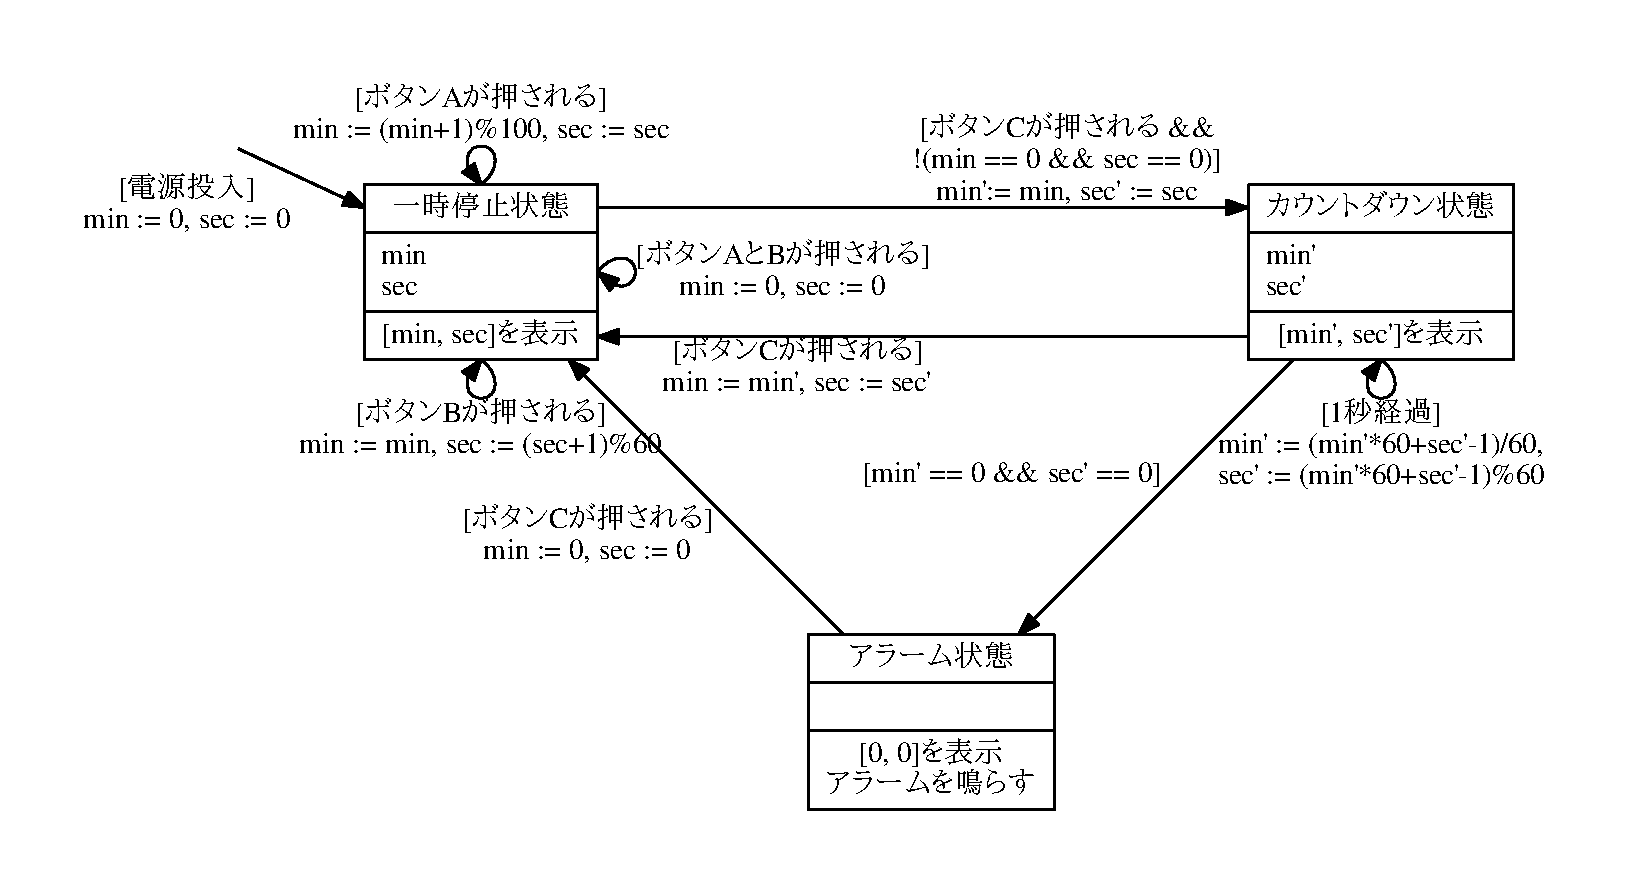
\includegraphics[width=155mm]{figure/ktimer_state.pdf}
 \end{center}
 \caption{KTIMERの状態遷移図}
 \label{fig:ktimer:state}
\end{figure}

\clearpage
\section{ハードウェア}
KTIMERのハードウェア仕様を図\ref{fig:ktimer:hardware}に簡単に示す。
この仕様に基づいてKTIMERの回路図を構成すると図\ref{fig:ktimer:circuit}の様になる。
図\ref{fig:ktimer:picture}はこの回路をブレッドボード上に実装した様子である。
実装に際し、電源電圧Vinの値はマイクロコントローラの動作電圧に合わせて5Vとした。
また、プルダウン抵抗R1の値は1k$\Omega$とし、制限抵抗R2の値は使用するLEDの最大許容電流との兼ね合いから200$\Omega$とした。

\begin{figure}[h]
\begin{screen}
\begin{itemize}
  \item マイクロコントローラにはAVR ATmega8を使用する。
  \item 時間の表示には4桁のカソードコモンの7セグメント表示器を用いてダイナミック点灯を行う。
  \item ボタンA、ボタンB、ボタンCにはそれぞれタクトスイッチを用いる。
  \item ブザーには圧電ブザーを用いる。
\end{itemize}
\end{screen}
\caption{KTIMERのハードウェア仕様}
\label{fig:ktimer:hardware}
\end{figure}

\begin{figure}[h]
 \begin{center}
  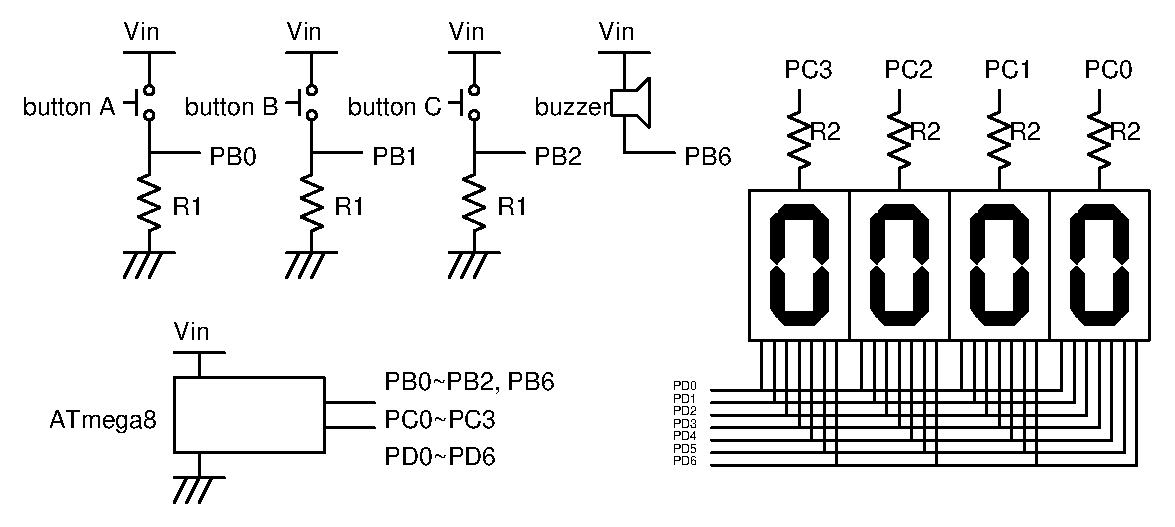
\includegraphics[width=160mm]{figure/circuit.ps}
 \end{center}
 \caption{KTIMERの回路図}
 \label{fig:ktimer:circuit}
\end{figure}

\begin{figure}[h]
 \begin{center}
  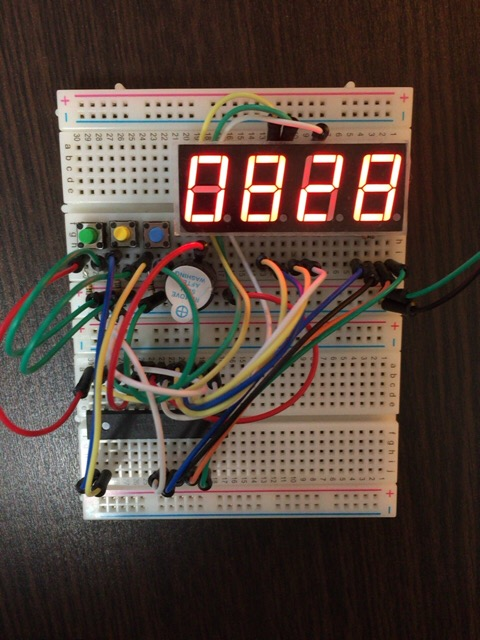
\includegraphics[scale=0.8]{figure/craft.jpg}
 \end{center}
 \caption{ブレッドボード上のKTIMER実装}
 \label{fig:ktimer:picture}
\end{figure}

\clearpage
\section{ソフトウェア}
Code \ref{code:ktimer:sfrp}は、SFRPによって記述したKTIMERプログラムである。
1行目から3行目において標準ライブラリをインポートしている。
以下にこれらの概要を示す。

\begin{itemize}
  \item \texttt{import Base}\\
  \texttt{Base}は各種演算子やタプル等の基本的な代数的データ構造を利用するためのライブラリである。
  整数型や整数リテラルなどもここで定義されており、ほぼ全てのSFRPプログラムは\texttt{Base}をインポートすることとなる。

  KTIMERプログラムの48行目に出現する演算子\texttt{>->}はC言語の\texttt{,}演算子と同じ意味を持つもので、
  左項の値を捨てて右項の値を返す。
  KTIMERプログラム中のその他の演算子は全てC言語における同名の演算子と同じ意味を持つものである。

  \item \texttt{import Base.AVR.ATMEGA8.GPIO as IO}\\
  \texttt{Base.AVR.ATMEGA8.GPIO}はATmega8が搭載するI/Oポートにアクセスするためのライブラリである。
  ノード\texttt{@pinXn}はポートPXnの時変値であり、
  \texttt{@posEdgePXn}はポートPXnの立ち上がり(PXnがHighになった瞬間のみTrueとなる)を表す時変値である。
  I/O関数\texttt{\$portX(n:Int, b:Bool):Unit}はポートPXnにbを出力し、
  \texttt{\$portXs(b:Int):Unit}はポート[PX7:PX0]にbを出力する。

  \item \texttt{import Base.AVR.ATMEGA8.Timer as Timer}\\
  \texttt{Base.AVR.ATMEGA8.Timer}はATmega8が搭載するタイマーを利用するためのライブラリである。
  \texttt{@dsec}は前回のイテレーションからの秒単位の経過時間であり、
  \ref{sec:language:model:program}項における時変値$\Delta t$の具体形であると言える。
\end{itemize}


\clearpage
\lstinputlisting[basicstyle=\ttfamily\small,language=SFRP,tabsize=2,caption={KTIMERのSFRPプログラム},label={code:ktimer:sfrp}]{./code/case-study/KTIMER.sfrp}

\section{実行性能}
\ref{sec:implementation:performance}節と同じ条件で実行形式の生成および実行性能の評価を行う。
すなわちavr-gccを用いてバイナリを生成し、メモリ使用量の見積もりと実行速度の測定を行う。
使用したSFRPコンパイラのバージョンは1.5.2、
avr-gccのバージョンは4.9.2である。

\subsection{メモリ性能}
生成されたSFRPの実行形式において、スタック使用量が最大となる関数コールパスを図\ref{fig:ktimer:call_graph}に示す。
ただし関数名の右横の数字はその関数で導入される局所変数のバイトサイズである。
\ref{sec:implementation:performance}節と同様に1回の関数呼び出しで消費するスタック領域を
\begin{center}
$スタックポインタを格納する2バイト領域 + 局所変数を格納する領域$
\end{center}
であると仮定すると、図\ref{fig:ktimer:call_graph}より最大スタック使用量は
\begin{center}
$(2 + 14) + (2 + 8) + (2 + 0) + (2 + 4) + (2 + 0) + (2 + 5) =$ 43 byte\\
\end{center}
であると算出される。


プログラムサイズおよび静的データサイズをavr-sizeコマンドによって調べた結果と合わせると表\ref{fig:ktimer:size}に示す通りとなる。
これにより、 KTIMERのFlushの使用量は1858byte、RAMの最大使用量は$45+43=$88byteであると算出される。
このメモリ使用量は、ATmega8を含む低価格帯のマイクロコントローラにとって十分に許容範囲内であると言える。

参考までに、C言語のみを用いてKTIMERを実装し、実行形式を生成してメモリ使用量の測定を行ったところ、
表\ref{fig:ktimer:naive:size}に示す結果となった。
ただし、使用したCコンパイラ及びコンパイルオプションは本節においてSFRPコンパイラがバイナリ生成のために
使用したものと同じである。
また、入出力処理に関してはSFRPコンパイラによって標準ライブラリとして提供され、
Code \ref{code:ktimer:sfrp}においても利用されているATmega8向けの入出力関数を
そのまま利用した。

\begin{figure}[h]
 \begin{center}
  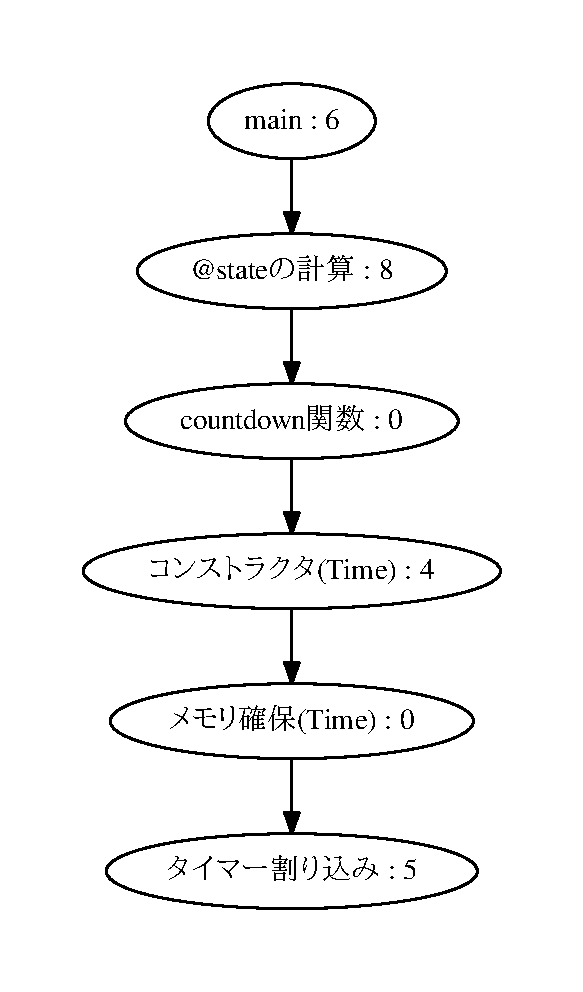
\includegraphics[width=60mm]{figure/call_graph_ktimer.pdf}
 \end{center}
 \caption{スタック使用量が最大となるKTIMERの実行形式の関数コールパス}
 \label{fig:ktimer:call_graph}
\end{figure}

\begin{table}[h]
  \centering
  \begin{tabular}{l|r}
    Programサイズ(avr-sizeコマンドより) & 1858 byte \\ \hline
    Dataサイズ(avr-sizeコマンドより) & 45 byte \\ \hline
    最大スタックサイズ(-fstack-usageオプションおよび手計算により算出)  & 43 byte \\ \hline
  \end{tabular}
\caption{KTIMERのメモリ使用量}
\label{fig:ktimer:size}
\end{table}

\begin{table}[h]
  \centering
  \begin{tabular}{l|r}
    Programサイズ(avr-sizeコマンドより) & 1206 byte \\ \hline
    Dataサイズ(avr-sizeコマンドより) & 42 byte \\ \hline
    最大スタックサイズ(-fstack-usageオプションおよび手計算により算出)  & 17 byte \\ \hline
  \end{tabular}
\caption{KTIMERをC言語のみを用いて記述した場合のメモリ使用量}
\label{fig:ktimer:naive:size}
\end{table}

\subsection{速度性能}
\ref{sec:implementation:performance:speed}項と同じ手法を用いて速度性能の計測を行うために、
Code \ref{code:ktimer:sfrp:bench}に示す記述をCode \ref{code:ktimer:sfrp}の末尾に追記する。
これにより、KTIMERの\texttt{PB7}番のI/Oポートを観測することによってイテレーション10000回当りの所要時間を求めることができる。

計測の結果は表\ref{fig:ktimer:time}に示す通りとなった。
イテレーション10000回に要する時間はBLINKLEDのそれと比べて約10倍であり、
イテレーション1回の所要時間は約3ミリ秒となることが分かる。
3ミリ秒という値はヒューマンインターフェースの反応時間としては十分であり、KTIMERは問題なく動作することができる。

\lstinputlisting[basicstyle=\ttfamily\small,language=SFRP,tabsize=2,caption={処理時間を計測するための追加記述},label={code:ktimer:sfrp:bench}]{./code/case-study/bench.sfrp}

\begin{table}[h]
  \centering
  \begin{tabular}{l|r}
    一時停止状態で動作させた場合 & \input{code/case-study/evaluation_wait/result1.txt} ミリ秒 \\ \hline
    カウントダウン状態で動作させた場合 & \input{code/case-study/evaluation_tick/result1.txt} ミリ秒 \\ \hline
  \end{tabular}
\caption{KTIMERのイテレーション10000回あたりの所要時間}
\label{fig:ktimer:time}
\end{table}

\chapter{記述性と実用性}
\section{代数的データ構造とパターンマッチ}
\section{シームレスな時変値プログラミング}
\section{再帰の禁止}
\section{破壊的な変更の禁止}
\section{外部ノード定義とノード出力定義}
\section{通常関数とI/O関数}
\section{外部定義}

\chapter{関連研究}
\section{Elm}
\section{RxCpp}
\section{EsterelとCeu}
\section{Simulink}
\section{CFRPとJuniper}
\section{Emfrp}

\chapter{結論}
\section{まとめ}
本研究では、マイクロコントローラにおいて実行されることを前提とした独自のFRP言語を考案し、そのコンパイラを実装した。
実例研究として、実際にこのコンパイラを用いて実用的な組み込みシステムを開発し、実行時性能の評価を行った。
最後に本言語の記述性と実用性についての議論を行い、既存の研究との関連についても述べた。

\section{今後の課題}

%\subsection{反復的な処理の記述をサポート}

\subsection{無名関数および第一級関数}
無名関数及び第一級関数をSFRP言語に導入することは可能である。
ただし現状の第一級でない関数と同様、再帰に関しては制限を受けることになる。
% また、クロージャは束縛される局所変数の個数に依存してデータサイズが決まるため、
% 代数的データ構造のように単純に型からデータサイズを特定することができず、
% \ref{sec:language:memory}節における評価を直接適用することはできない。
% 実装に際してはこの点について何らかの対処が必要になるだろう。

\subsection{任意の場所での初期値定義}
現状のSFRPではトップレベルに定義される時変値であるノードに対してのみ、初期値の定義及び直前値の参照が許されている。
これは\ref{sec:language:model}節における計算モデルには存在しない制約であり、
SFRPにとっても本質的に必要とされる制約ではない。
この制約が存在しなければ、時変値に対して初期値を付与する関数や時変値の直前値を参照する関数などを定義することが可能となり、
時変値に関する定形処理の記述が容易になる。
ただし動的メモリ確保を排除する現在の設計方針の元でこの制約を撤廃することは、
コンパイラ実装の観点から見れば容易ではないと予想される。

% \subsection{外部ノードの定義に変数を許す}
% 多くのマイクロコントローラにおいてメモリマップドI/Oによる入出力インターフェースが採用されていることから、
% 外部ノード定義の入力源に直接これを指定できるようになれば大変便利である。

\subsection{内部ポーリングの手動制御}
現状のSFRPでは、時変値更新のための内部ポーリングを自由に制御することはできない。
このため、システムをスリープモードへ移行させる処理などを記述することは難しいと思われる。
また、時変値更新のタイミングをユーザが独自に制御したいというケースもあるかもしれない。
内部ポーリングの手動制御を実施するインターフェースを言語内に導入すれば、そういったニーズに応えることができると思われる。

\chapter*{謝辞}
最後に書く。

\bibliographystyle{abbrv}
\bibliography{tex/reference}
\end{document}
